\documentclass[aspectratio=169,11pt]{beamer}
\usetheme{Madrid}
\usecolortheme{whale}
\definecolor{uddblue}{HTML}{1F4E79}
\definecolor{uddlight}{HTML}{2E86C1}
\setbeamercolor{structure}{fg=uddblue}
\setbeamercolor{frametitle}{bg=uddblue,fg=white}
\setbeamercolor{title}{bg=uddblue,fg=white}
\setbeamercolor{block title}{bg=uddblue,fg=white}
\setbeamercolor{block body}{bg=uddblue!10}
\setbeamercolor{item}{fg=uddblue}
\usepackage[utf8]{inputenc}
\usepackage[T1]{fontenc}
\usepackage[english]{babel}
\usepackage{amsmath,amssymb}
\usepackage{graphicx}
\usepackage{booktabs}
\usepackage{listings}
\usepackage{tikz}
\usetikzlibrary{shapes,arrows,positioning,calc}

ewcommand{\xmark}{\textcolor{red}{\texttimes}}
\newcommand{\cmark}{\textcolor{green!60!black}{\checkmark}}
\lstset{language=R,basicstyle=\ttfamily\scriptsize,keywordstyle=\color{uddblue}\bfseries,commentstyle=\color{gray},stringstyle=\color{uddlight},backgroundcolor=\color{uddblue!5},frame=single,rulecolor=\color{uddblue!30},breaklines=true,showstringspaces=false}
\graphicspath{{figuras/}}
\titlegraphic{
\includegraphics[height=1.2cm]{logo_gobierno.png}}
\institute[CICS — UDD]{Doctorado en Ciencias de la Complejidad Social — CICS, UDD}
\date{19 de marzo de 2026}

\title{Sesión 4: Inferencia Estadística — Estimación}
\author[A. Agüero]{Amaru Agüero}

\begin{document}

\begin{frame}[plain]
\titlepage
\end{frame}

% ====================================================================
% SLIDE 1: AGENDA
% ====================================================================
\begin{frame}{Agenda}
\tableofcontents
\end{frame}

% ====================================================================
% SECTION 1: LÓGICA DE LA INFERENCIA
% ====================================================================
\section{Lógica de la Inferencia}

\begin{frame}{¿Por qué hacemos inferencia estadística?}
\begin{itemize}
  \item Raramente podemos observar toda la \textbf{población}
  \pause
  \item Estudiamos una \textbf{muestra} para aprender sobre el todo
  \pause
  \item La pregunta central: ¿Qué podemos decir sobre la población con base en la muestra?
  \pause
  \item \textbf{Dos enfoques principales:}
  \begin{enumerate}
    \item Estimación puntual: Proponer un único valor para el parámetro
    \item Estimación por intervalo: Construir un rango plausible
  \end{enumerate}
\end{itemize}
\end{frame}

\begin{frame}{Parámetro vs. Estadístico}
\begin{columns}[T]
\column{0.45\textwidth}
\textbf{Parámetro} (población)
\begin{itemize}
  \item $\mu$ = media poblacional
  \item $\sigma$ = desv. estándar poblacional
  \item $\sigma^2$ = varianza poblacional
  \item $p$ = proporción poblacional
  \item $\rho$ = correlación poblacional
  \pause
  \item \textcolor{red}{Desconocido} (típicamente)
  \item \textcolor{red}{Fijo}
\end{itemize}

\column{0.45\textwidth}
\textbf{Estadístico} (muestra)
\begin{itemize}
  \item $\bar{x}$ = media muestral
  \item $s$ = desv. estándar muestral
  \item $s^2$ = varianza muestral
  \item $\hat{p}$ = proporción muestral
  \item $r$ = correlación muestral
  \pause
  \item \textcolor{uddblue}{Conocido} (calculado)
  \item \textcolor{uddblue}{Varía} entre muestras
\end{itemize}
\end{columns}
\end{frame}

\begin{frame}{Distribución Muestral: El Concepto Clave}
\small
\begin{block}{¿Qué es?}
La distribución de probabilidad de un estadístico (ej.\ $\bar{x}$) calculado en todas las posibles muestras de tamaño $n$.
\end{block}

\pause

\begin{center}
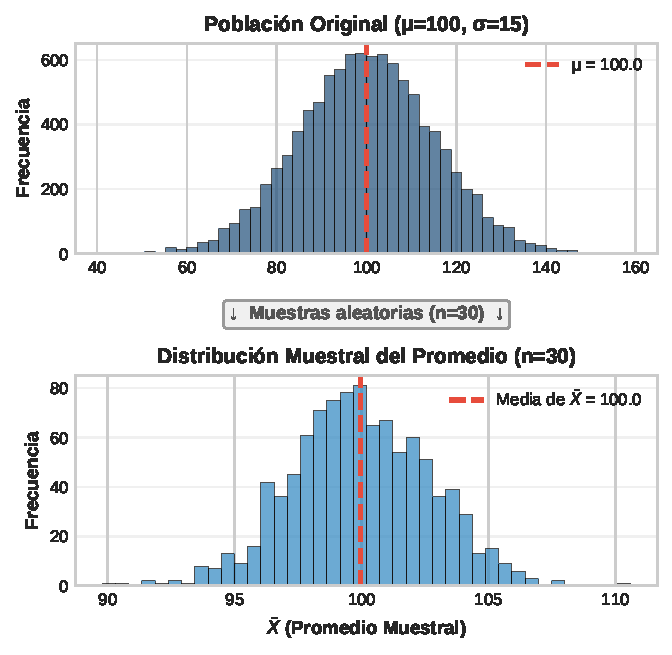
\includegraphics[width=0.7\textwidth,height=0.45\textheight,keepaspectratio]{distribucion_muestral.pdf}
\end{center}

\pause
\vspace{-0.2cm}
\begin{itemize}\setlength{\itemsep}{0pt}
  \item La distribución muestral es más \textbf{concentrada} que la poblacional
  \item Su centro es el parámetro poblacional; su dispersión depende de $n$
\end{itemize}
\end{frame}

\begin{frame}{Error Estándar}
\small
\begin{block}{Definición}
El error estándar (SE) es la desviación estándar de la distribución muestral de un estadístico.
\end{block}

\pause

\textbf{Para la media muestral:} \quad $SE_{\bar{x}} = \dfrac{\sigma}{\sqrt{n}}$

\pause
\vspace{0.2cm}

\textbf{Implicaciones:}
\begin{itemize}\setlength{\itemsep}{0pt}
  \item El SE disminuye con $\sqrt{n}$ (no es lineal)
  \item Muestras más grandes $\Rightarrow$ estimadores más precisos
  \item Duplicar $n$ reduce el SE en $\approx 30\%$; el SE aumenta con $\sigma$
\end{itemize}

\pause
\vspace{0.1cm}

\begin{alertblock}{Nota importante}
En la práctica, $\sigma$ es desconocida. Estimamos $SE$ usando $s$ (desv.\ est.\ muestral).
\end{alertblock}
\end{frame}

% ====================================================================
% SECTION 2: ESTIMACIÓN PUNTUAL
% ====================================================================
\section{Estimación Puntual}

\begin{frame}{¿Qué es un buen estimador?}
\begin{block}{Propiedades deseables}
\begin{enumerate}
  \item \textbf{Insesgamiento:} $E[\hat{\theta}] = \theta$ (en promedio, acertamos)
  \pause
  \item \textbf{Eficiencia:} Varianza pequeña (precisión)
  \pause
  \item \textbf{Consistencia:} Conforme $n \to \infty$, $\hat{\theta} \to \theta$
\end{enumerate}
\end{block}

\pause

\begin{columns}[T]
\column{0.45\textwidth}
\textbf{Insesgado pero ineficiente}
\begin{center}
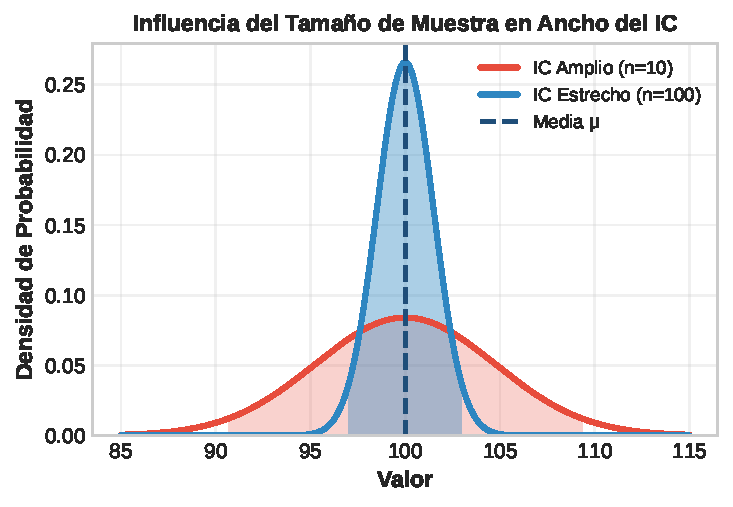
\includegraphics[width=0.85\linewidth,height=0.4\textheight,keepaspectratio]{ancho_ic.pdf}
\end{center}

\column{0.45\textwidth}
\textbf{Eficiente e insesgado}
\begin{center}
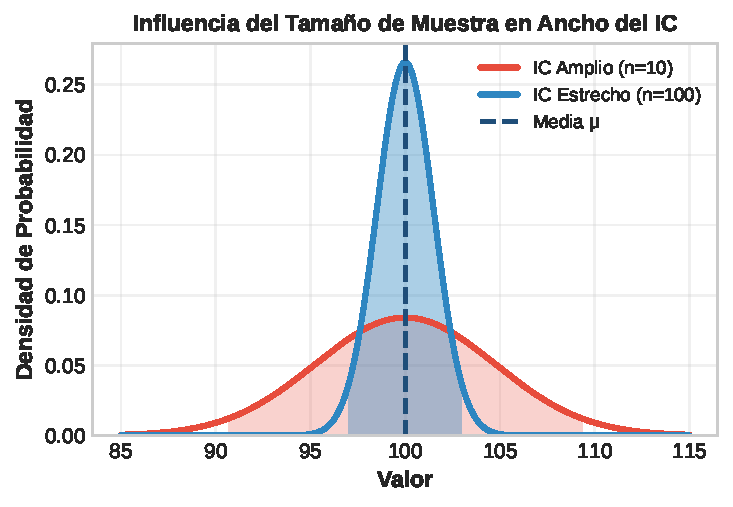
\includegraphics[width=0.85\linewidth,height=0.4\textheight,keepaspectratio]{ancho_ic.pdf}
\end{center}
\end{columns}

\end{frame}

\begin{frame}{La Media Muestral como Estimador}
\small
\begin{block}{Propiedades de $\bar{x}$}
\begin{itemize}\setlength{\itemsep}{1pt}
  \item \textbf{Insesgado}: $E[\bar{x}] = \mu$
  \pause
  \item \textbf{Consistente}: $\bar{x} \xrightarrow{p} \mu$ (ley de los grandes números)
  \pause
  \item \textbf{Distribución muestral}: $\bar{x} \sim N\!\left(\mu, \frac{\sigma^2}{n}\right)$
  \pause
  \item \textbf{TLC}: Incluso si $X$ no es normal, $\bar{x}$ es aprox.\ normal para $n$ grande
\end{itemize}
\end{block}

\pause
\vspace{0.1cm}

\begin{exampleblock}{Ejemplo}
Si $\mu = 100$, $\sigma = 15$, $n = 100$: $SE_{\bar{x}} = 1.5$. El 95\% de las medias caerán en $(97.06,\; 102.94)$.
\end{exampleblock}
\end{frame}

\begin{frame}{La Proporción Muestral como Estimador}
\small
\begin{block}{Propiedades de $\hat{p}$}
\begin{itemize}\setlength{\itemsep}{1pt}
  \item \textbf{Insesgado}: $E[\hat{p}] = p$
  \pause
  \item Distribución muestral (aprox.): $\hat{p} \sim N\!\left(p, \frac{p(1-p)}{n}\right)$
  \pause
  \item Error estándar: $SE_{\hat{p}} = \sqrt{\frac{p(1-p)}{n}}$
  \pause
  \item Condición: $np > 5$ y $n(1-p) > 5$
\end{itemize}
\end{block}

\pause
\vspace{0.1cm}

\begin{exampleblock}{Ejemplo}
Muestra de 500 personas, 280 apoyan cierta política: $\hat{p} = 0.56$, $SE_{\hat{p}} = \sqrt{\frac{0.56 \times 0.44}{500}} = 0.022$.
\end{exampleblock}
\end{frame}

\begin{frame}{Máxima Verosimilitud: Intuición}
\small
\begin{block}{Idea central}
Elegir el parámetro $\hat{\theta}$ que hace \textit{más probable} observar los datos que tenemos.
\end{block}

\pause

\begin{example}
Lanzamos una moneda 10 veces y observamos 8 caras. ¿Es justa?
\begin{itemize}\setlength{\itemsep}{0pt}
  \item Si $p = 0.5$ (justa): $P(\text{8 caras}) = 0.044$
  \item Si $p = 0.8$: $P(\text{8 caras}) = 0.302$
  \pause
  \item \textbf{Estimador MV:} $\hat{p}_{MV} = 8/10 = 0.8$ (hace más probable lo observado)
\end{itemize}
\end{example}

\pause

\begin{alertblock}{Conexión}
Para $\bar{x}$ y $\hat{p}$, el estimador de MV coincide con el estimador insesgado.
\end{alertblock}
\end{frame}

% ====================================================================
% SECTION 3: INTERVALOS DE CONFIANZA
% ====================================================================
\section{Intervalos de Confianza}

\begin{frame}{Construcción General de un IC}
\begin{block}{Fórmula}
\begin{equation*}
\text{IC} = \text{Estimador} \pm z^* \times SE
\end{equation*}
\end{block}

\pause
\small
\begin{columns}[T]
\column{0.5\textwidth}
\begin{itemize}\setlength{\itemsep}{0pt}
  \item \textbf{Estimador}: $\bar{x}$, $\hat{p}$, $\hat{\beta}$, etc.
  \pause
  \item \textbf{$z^*$}: Valor crítico
  \begin{itemize}\setlength{\itemsep}{0pt}
    \item 95\% con $Z$: $z^* = 1.96$
    \item 99\% con $Z$: $z^* = 2.576$
    \item 95\% con $t$: $z^* = t_{\alpha/2, n-1}$
  \end{itemize}
  \pause
  \item \textbf{SE}: Error estándar del estimador
\end{itemize}

\column{0.5\textwidth}
\pause
\begin{center}
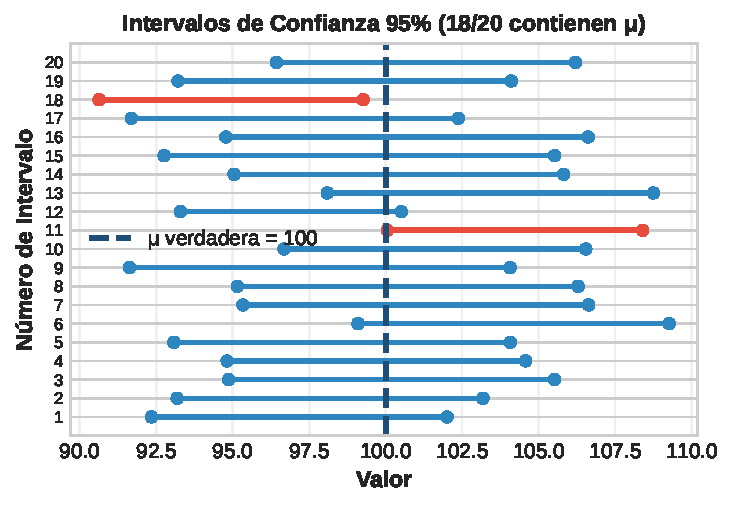
\includegraphics[width=\linewidth,height=0.55\textheight,keepaspectratio]{intervalo_confianza.pdf}
\end{center}
\end{columns}
\end{frame}

\begin{frame}{IC para la Media: $\sigma$ Conocida}
\small
\begin{block}{Supuestos}
Muestra aleatoria de población normal (o $n$ grande); $\sigma$ conocida (raro en la práctica).
\end{block}

\pause

\begin{block}{IC al $(1-\alpha) \times 100\%$}
$\bar{x} \pm z_{\alpha/2} \cdot \frac{\sigma}{\sqrt{n}}$
\end{block}

\pause

\begin{exampleblock}{Ejemplo}
$n = 100$, $\bar{x} = 45.2$, $\sigma = 8$. IC 95\%: $45.2 \pm 1.96 \times \frac{8}{\sqrt{100}} = 45.2 \pm 1.568 = (43.63,\; 46.77)$
\end{exampleblock}

\pause

\begin{alertblock}{En la práctica: $\sigma$ desconocida}
Reemplazamos $\sigma$ por $s$ y usamos distribución $t$: \quad $\bar{x} \pm t_{\alpha/2, n-1} \cdot \frac{s}{\sqrt{n}}$
\end{alertblock}
\end{frame}

\begin{frame}{IC para la Media: $\sigma$ Desconocida (caso usual)}
\small
\begin{block}{Supuestos}
Muestra aleatoria de población normal (importante si $n < 30$); $\sigma$ desconocida (típico).
\end{block}

\pause

\begin{block}{IC al $(1-\alpha) \times 100\%$}
$\bar{x} \pm t_{\alpha/2, n-1} \cdot \frac{s}{\sqrt{n}}$
\end{block}

\pause

\begin{itemize}\setlength{\itemsep}{0pt}
  \item $t$ tiene colas más pesadas que la normal; $n \to \infty \Rightarrow t_{n-1} \to Z$
  \pause
  \item Para $n \geq 30$, la aproximación normal es aceptable
\end{itemize}

\pause

\begin{exampleblock}{Ejemplo}
$n = 25$, $\bar{x} = 52.3$, $s = 6.5$, $t_{0.025, 24} = 2.064$. IC 95\%: $52.3 \pm 2.064 \times \frac{6.5}{\sqrt{25}} = 52.3 \pm 2.68 = (49.62,\; 54.98)$
\end{exampleblock}
\end{frame}

\begin{frame}{IC para una Proporción}
\small
\begin{block}{Método de Wald (simple)}
$\hat{p} \pm z_{\alpha/2} \cdot \sqrt{\frac{\hat{p}(1-\hat{p})}{n}}$
\end{block}

\pause

\begin{alertblock}{Limitación del Wald}
Funciona mal cuando $\hat{p}$ es cercana a 0 o 1 (intervalos negativos o $>1$).
\end{alertblock}

\pause

\begin{block}{Método de Wilson (corrección recomendada)}
\scriptsize
$\frac{\hat{p} + \frac{z_{\alpha/2}^2}{2n}}{1 + \frac{z_{\alpha/2}^2}{n}} \pm \frac{z_{\alpha/2}}{1 + \frac{z_{\alpha/2}^2}{n}} \sqrt{\frac{\hat{p}(1-\hat{p})}{n} + \frac{z_{\alpha/2}^2}{4n^2}}$
\end{block}

\pause

\begin{exampleblock}{Ejemplo}
$n = 200$, $\hat{p} = 0.175$. Wald IC 95\%: $0.175 \pm 1.96\sqrt{\frac{0.175 \times 0.825}{200}} = (0.105,\; 0.245)$. Wilson es más preciso para $\hat{p}$ extremas.
\end{exampleblock}
\end{frame}

\begin{frame}{IC para Diferencia de Dos Medias}
\begin{columns}[T]
\column{0.55\textwidth}
\textbf{Supuesto: Varianzas iguales}
\begin{equation*}
(\bar{x}_1 - \bar{x}_2) \pm t_{\alpha/2, n_1+n_2-2} \cdot SE
\end{equation*}

donde
\begin{equation*}
SE = s_p \sqrt{\frac{1}{n_1} + \frac{1}{n_2}}
\end{equation*}

\column{0.45\textwidth}
\textbf{Supuesto: Varianzas desiguales}
\begin{equation*}
(\bar{x}_1 - \bar{x}_2) \pm t_{\alpha/2, df} \cdot SE
\end{equation*}

donde
\begin{equation*}
SE = \sqrt{\frac{s_1^2}{n_1} + \frac{s_2^2}{n_2}}
\end{equation*}
\end{columns}

\pause

\vspace{0.3cm}

\begin{exampleblock}{Interpretación}
Si el IC contiene 0, no hay diferencia significativa entre los grupos.
\end{exampleblock}
\end{frame}

% ====================================================================
% SECTION 4: INTERPRETACIÓN DE IC
% ====================================================================
\section{Interpretación Correcta del IC}

\begin{frame}{¿Qué significa realmente un IC 95\%?}
\small
\begin{block}{Interpretación frecuentista CORRECTA}
``Si repitiéramos el muestreo muchas veces, aproximadamente el 95\% de los IC contendrían al parámetro verdadero.''
\end{block}

\pause

\begin{alertblock}{Interpretación INCORRECTA (muy común)}
\begin{itemize}\setlength{\itemsep}{0pt}
  \item ``Hay 95\% de probabilidad de que $\mu$ esté en este intervalo'' \textcolor{red}{\xmark}
  \item ``El parámetro tiene 95\% de probabilidad de estar aquí'' \textcolor{red}{\xmark}
  \item ``El 95\% de los datos cae en este intervalo'' \textcolor{red}{\xmark}
\end{itemize}
\end{alertblock}

\pause

\begin{block}{¿Por qué es incorrecta?}
Una vez construido el IC, $\mu$ está \textbf{dentro} o \textbf{fuera}. La probabilidad 0.95 se refiere al proceso de muestreo repetido, no al intervalo específico.
\end{block}
\end{frame}

\begin{frame}{Factores que Afectan el Ancho del IC}
\small
\begin{columns}[T]
\column{0.48\textwidth}
\textbf{Aumentan el ancho:}
\begin{itemize}\setlength{\itemsep}{0pt}
  \item \textcolor{red}{Menor $n$}
  \item \textcolor{red}{Mayor variabilidad} ($\sigma \uparrow$)
  \item \textcolor{red}{Mayor confianza} (95\% vs 90\%)
\end{itemize}

\vspace{0.1cm}
\begin{center}
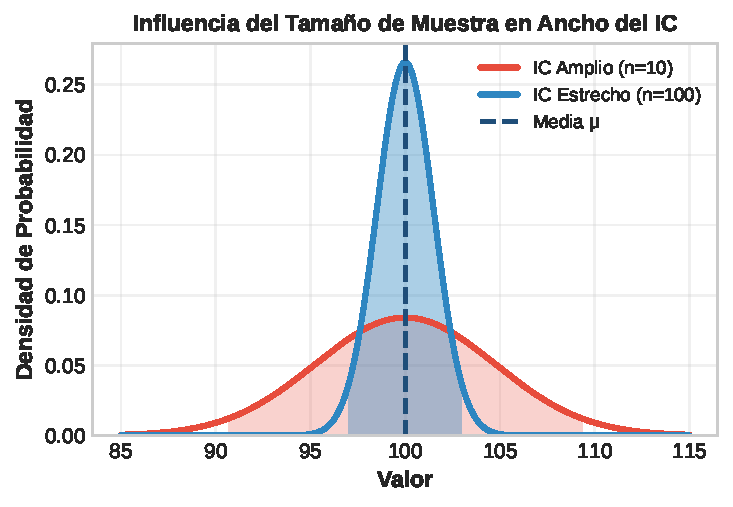
\includegraphics[width=\linewidth,height=0.4\textheight,keepaspectratio]{ancho_ic.pdf}
\end{center}

\column{0.48\textwidth}
\textbf{Disminuyen el ancho:}
\begin{itemize}\setlength{\itemsep}{0pt}
  \item \textcolor{uddblue}{Mayor $n$}
  \item \textcolor{uddblue}{Menor variabilidad} ($\sigma \downarrow$)
  \item \textcolor{uddblue}{Menor confianza} (90\% vs 95\%)
\end{itemize}

\vspace{0.1cm}
\begin{center}
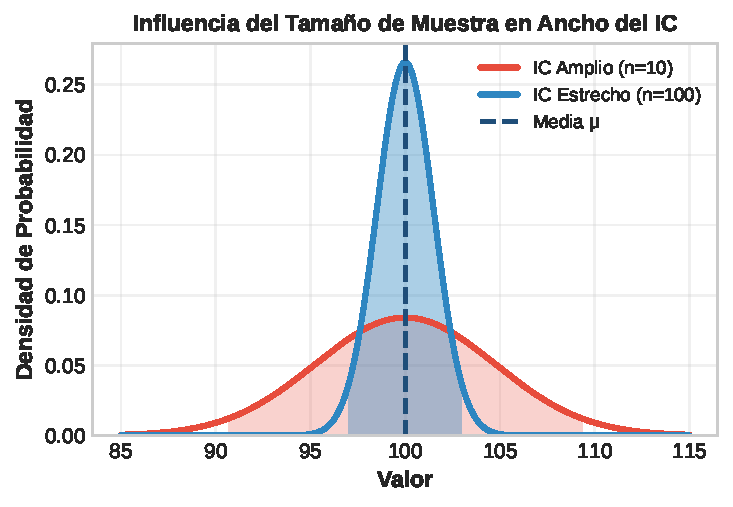
\includegraphics[width=\linewidth,height=0.4\textheight,keepaspectratio]{ancho_ic.pdf}
\end{center}
\end{columns}

\pause
\vspace{-0.1cm}
\begin{alertblock}{Trade-off}
Más confianza $\Leftrightarrow$ intervalo más amplio. No podemos tener ambas sin más datos.
\end{alertblock}
\end{frame}

% ====================================================================
% SECTION 5: R EN LA PRÁCTICA
% ====================================================================
\section{Implementación en R}

\begin{frame}[fragile]{Intervalo de Confianza para la Media: t.test()}
\begin{lstlisting}
# Datos de ejemplo
datos <- c(23.5, 24.1, 22.8, 25.3, 23.9, 24.6, 23.2)

# IC 95% para la media (con sigma desconocida)
resultado <- t.test(datos, conf.level = 0.95)
resultado$estimate      # Media muestral
resultado$conf.int      # Intervalo de confianza
resultado$statistic     # Estadístico t
resultado$p.value       # Valor p

# IC 99%
t.test(datos, conf.level = 0.99)$conf.int
\end{lstlisting}

\pause

\begin{exampleblock}{Salida típica}
\verb|95 percent confidence interval:|
\verb| 22.88571 25.01429|
\end{exampleblock}
\end{frame}

\begin{frame}[fragile]{Intervalo de Confianza para una Proporción}
\begin{lstlisting}
# Proporción de éxitos: 35 de 200
prop.test(x = 35, n = 200, conf.level = 0.95)

# Resultado incluye IC usando método de Wilson
# $estimate: 0.175
# $conf.int: [0.1241, 0.2359] (aproximadamente)

# Para una sola proporción (más flexible)
binom.test(x = 35, n = 200, p = 0.5,
           conf.level = 0.95)
# Usa distribución binomial exacta

# IC directa (Clopper-Pearson, exacta)
binom.confint(x = 35, n = 200,
              method = "clopper-pearson")
\end{lstlisting}

\pause

\begin{alertblock}{Nota}
\verb|prop.test()| usa Wilson. \verb|binom.test()| usa exacta (Clopper-Pearson).
\end{alertblock}
\end{frame}

\begin{frame}[fragile]{Simulación: Distribución de Intervalos}
\begin{lstlisting}[basicstyle=\ttfamily\tiny]
# Simular 1000 muestras y sus IC 95%
set.seed(123)
n_sim <- 1000; n <- 50; mu <- 100; sigma <- 15

# Almacenar IC
ics <- matrix(NA, n_sim, 2)

for (i in 1:n_sim) {
  muestra <- rnorm(n, mu, sigma)
  ic <- t.test(muestra)$conf.int
  ics[i, ] <- ic
}

# Contar cuántos IC contienen mu
cubiertos <- sum(ics[, 1] <= mu & mu <= ics[, 2])
cat("IC que contienen mu:", cubiertos/n_sim)
# Esperado: aprox 0.95
\end{lstlisting}

\pause
\small
\begin{block}{Verificación}
Demuestra que el 95\% de los intervalos contiene realmente el parámetro.
\end{block}
\end{frame}

\begin{frame}[fragile]{IC para Diferencia de Medias: t.test()}
\begin{lstlisting}
# Dos muestras independientes
grupo1 <- c(23.5, 24.1, 22.8, 25.3, 23.9)
grupo2 <- c(28.3, 29.1, 27.8, 30.2, 28.9)

# IC 95% para la diferencia de medias
t.test(grupo1, grupo2, conf.level = 0.95)

# Si varianzas desiguales (Welch)
t.test(grupo1, grupo2, var.equal = FALSE)

# Si varianzas iguales
t.test(grupo1, grupo2, var.equal = TRUE)

# Muestras pareadas
pre <- c(100, 95, 110, 105, 98)
post <- c(105, 100, 115, 110, 103)
t.test(pre, post, paired = TRUE)
\end{lstlisting}
\end{frame}

% ====================================================================
% SECTION 6: EJERCICIO PRÁCTICO
% ====================================================================
\section{Ejercicio Práctico}

\begin{frame}{Ejercicio Práctico}
\begin{block}{Contexto}
Se desea estimar el promedio de \textbf{ingresos mensuales} de egresados del programa de Doctorado en Ciencias de la Complejidad Social. Se toma una muestra aleatoria de 40 egresados.
\end{block}

\pause

\vspace{0.3cm}

\begin{exampleblock}{Datos (simulados)}
\begin{itemize}
  \item Muestra: $n = 40$
  \item Media muestral: $\bar{x} = \$2,450,000$ (CLP)
  \item Desviación estándar muestral: $s = \$380,000$
\end{itemize}
\end{exampleblock}

\pause

\vspace{0.3cm}

\textbf{Preguntas:}
\begin{enumerate}
  \item Construya un IC 95\% para el ingreso promedio poblacional
  \item Interprete el intervalo correctamente
  \item ¿Qué tamaño de muestra sería necesario para un IC con ancho de $\pm\$100,000$?
  \item ¿Cómo cambiaría el IC si usara confianza 99\%?
\end{enumerate}
\end{frame}

\begin{frame}[fragile]{Solución en R}
\begin{lstlisting}[basicstyle=\ttfamily\tiny]
# Datos
n <- 40; x_barra <- 2450000; s <- 380000

# IC 95% (usando distribución t)
alpha <- 0.05
t_crit <- qt(1 - alpha/2, df = n - 1)
SE <- s / sqrt(n)
margen <- t_crit * SE

ic_lower <- x_barra - margen
ic_upper <- x_barra + margen
cat("IC 95%: [", ic_lower, ",", ic_upper, "]", "\n")

# O usando t.test con datos simulados
set.seed(42)
datos_ingresos <- rnorm(n, x_barra, s)
t.test(datos_ingresos, conf.level = 0.95)$conf.int
\end{lstlisting}

\pause
\small
\begin{exampleblock}{Respuesta}
IC 95\% $\approx$ [\$2,327,549, \$2,572,451]
\end{exampleblock}
\end{frame}

\begin{frame}{Reflexión: ¿Por qué importa la inferencia?}
\begin{itemize}
  \item \textbf{Muestreo}: Casi nunca podemos estudiar la población completa
  \pause
  \item \textbf{Incertidumbre cuantificable}: Los IC nos dicen qué tan precisas son nuestras estimaciones
  \pause
  \item \textbf{Decisiones informadas}: Podemos distinguir entre variabilidad muestral y efectos reales
  \pause
  \item \textbf{Reproducibilidad}: Reportar IC (no solo estimadores) permite evaluar la confiabilidad
\end{itemize}

\pause

\vspace{0.4cm}

\begin{alertblock}{En la próxima sesión}
Haremos \textbf{pruebas de hipótesis}: contrastar afirmaciones sobre parámetros poblacionales usando muestras.
\end{alertblock}
\end{frame}

% ====================================================================
% CLOSING SLIDE
% ====================================================================
\begin{frame}[plain]
\begin{center}
\Huge \textcolor{uddblue}{¿Preguntas?}
\end{center}
\end{frame}

\end{document}
